\documentclass[letterpaper, 12pt]{article}

\usepackage{graphicx}
\usepackage{longtable}
\usepackage{rotating}
\usepackage{dcolumn}
\usepackage{listings}
\usepackage{subfiles}
\usepackage{amsmath}
\usepackage[margin=0.5in]{geometry} % for more room on the pages :)

% Code listing commands
\lstset{language=R,
basicstyle=\scriptsize\ttfamily,
commentstyle=\ttfamily,
numbers=left,
numberstyle=\footnotesize,
stepnumber=1,
numbersep=5pt,
showspaces=false,
showstringspaces=false,
showtabs=false,
frame=single,
tabsize=2,
captionpos=b,
breaklines=true,
breakatwhitespace=false,
title=\lstname,
escapeinside={},
keywordstyle={},
morekeywords={}
}

%TODO: change format so sections are numbered (1,2,3...) and subsections are Alpha (A,B,C....)
\renewcommand\thesection{Part \Alph{section}:}
\renewcommand\thesubsection{(\roman{subsection})}
\newcommand{\ind}[1]{\textbf{1}\{#1\}}

\graphicspath{{img/}}

\begin{document}
\title{ARE213 Problem Set \#3}
\author{Peter Alstone \& Frank Proulx}
\maketitle

\section{Linear models to motivate RD}

\subsection{LM results comparison}

\subfile{tab1a.tex}

Using a series of linear models (with heteroskedasticity consistent ``robust" standard errors), we find that for a range of model formulations there is a significant effect on housing price from the presence of hazardous waste cleanup sites with increased housing values in places with cleanup.  The coefficient for the hazardous waste cleanup indicator variable (npl2000) takes a wide range of values depending on which additional explanatory variables are included in the model, from 0.04 (i.e., approximately a 4\% increase) for the simple model only including 1980 housing values and npl2000 to estimate 2000 housing values, to 0.09 for a model including both housing and demographic characteristics.  

\paragraph{Requirements for Unbiased Estimates:}For our estimates to be unbiased we would need to include all of the potential sources of variation in housing price in a linear model.  A particular challenge is that there are very few sites with NPL2000 status (only 2\% of sites), so while the overall sample size is large there is very little support for estimates related to NPL2000 status compared to other covariates.  The overlap assumption must hold for the regression to be successful.  

\subsection{Comparing covariates}

We compare the covariates between census tracts and sites in a series of contingency tables and find that there are wide disparities between census tracts with and without NPL2000 status.  This erodes confidence that there is support in the data to use tract-level linear regression models, since the overlap assumption may be violated from wide differences in the other characteristics on the tract level.  On the site level, simply comparing over / under the trigger limit for the national priorities list (HRS score of 28.5) seems to solve some but not all the problems with overlap.  While many covariates cannot be said to come from different distributions there are still some that have significant differences.  Narrowing into a window from 16.5 - 40.5 (with the 28.5 dividing line) results in comparisons for which the hypothesis that the covariates are from the same distribution is not rejected.  Overall, these comparisons motivate the regression discontinuity design.  By narrowing in on a region where overlap in distribution for the covariates holds we have a fighting chance to identify a treatment effect, albeit with difficulty in establishing external validity.  

\subfile{tab1b-1.tex}
\subfile{tab1b-2.tex}
\subfile{tab1b-3.tex}

\section{RDD setup}

\subsection{HRS as running variable?}
To be a running variable HRS need to be continuous and not subject to manipulation around the boundary value.  If the variable is as good as random around the cutoff (which is based soley on its value) we can use a sharp RDD.  The ``facts" presented in the assignment tend to support the choice.  HRS was selected in rather capricious ways (``the 28.5 cutoff was selected...(for) a manageable number of sites"), was expected to be unknown to the people who generated the data, and is an imprecise (``imperfect") scoring indicator. 


\subsection{McCrary Test}
% NOTE: I flipped the interpretation here...we want continuity here and discontinuity when we plot HRS by the outcome (price).  
It does not appear that any manipulation occured around the threshold for listing on the NPL.  Based on the plot of the density distribution (Figure \ref{fig:ddplot}) using default values for bandwidth and bin width ($h \approx 12.6$, $b \approx 1.6$), there is no significant discontinuity in the neighborhood of HRS=28.5. The estimated value lines appear to nearly match with each other, and more importantly the upperbound 95\% C.I. for values below HRS=28.5 and the estimated value above HRS=28.5 overlap, and vice versa for the lowerbound 95\% C.I. for values above HRS = 28.5. This indicates the choice of HRS as a running variable in the RDD is appropriate. This lack of discontinuity appears to be consistent across various bandwidth values (tested with values $h = \{4, 8, 16, 20\}$).  

\begin{figure}[htbp]
\begin{center}
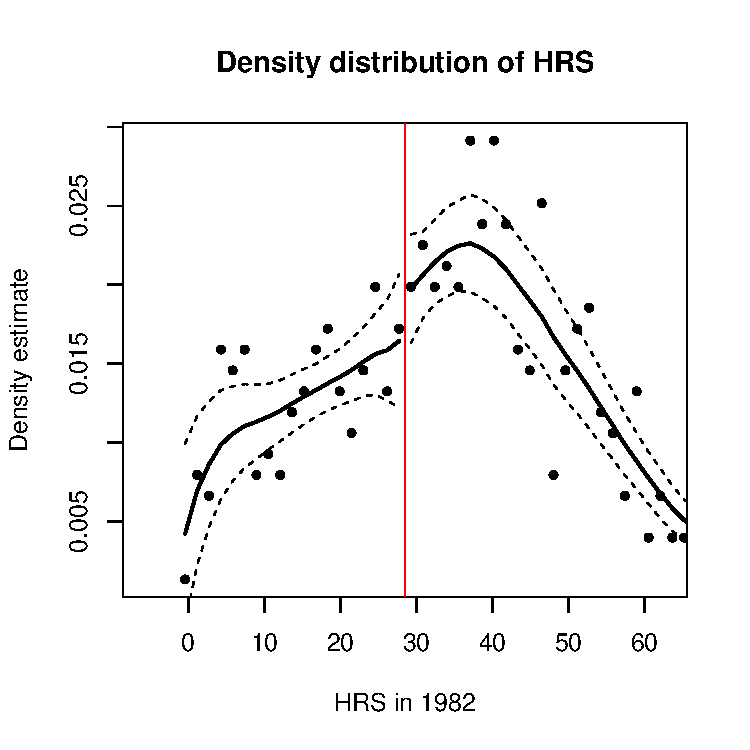
\includegraphics{ddplot.pdf}
\caption{Density distribution histogram for 1982 HRS.}
\label{fig:ddplot}
\end{center}
\end{figure}


\section{RDD First Stage}


\subsection{2SLS first stage specification}
The first stage equation is:

 $NPL_{2000}=\gamma_1\ind{HRS_{82} > 28.5} +\gamma_2(HRS_{82}-c) + \gamma_3(HRS_{82}-c)*\ind{HRS_{82} > 28.5}+x_i\gamma_4+u_i$.
 
 We use the full set of covariates ($x_i$) but not state level fixed effects in the analyses below.  Both the full dataset and a constrained linear regression around the threshold (plus or minus 12 points) show a statistically significant first stage.  Combined with the graphical analysis below we are confident that the first stage is useful for a fuzzy RD design.  

\subsection{Graphic: NPL and HRS scores}

Figure \ref{fig:3b} shows how presence on the NPL by 2000 depends very strongly, nearly ``sharply" on the value of the HRS score in 1982.  Only a handful of sites do not follow the strict cutoff rule.  As one would expect there are many more (but not exclusively) non-compliers with the strict boundary for cleanup on the low side of the cutoff, i.e., sites where the HRS score should not have resulted in listing.  Either a revised HRS score later than 1982 or some other change (including manipulation of the process, etc.) is responsible for these cases.  

\begin{figure}[htbp!]
\begin{center}
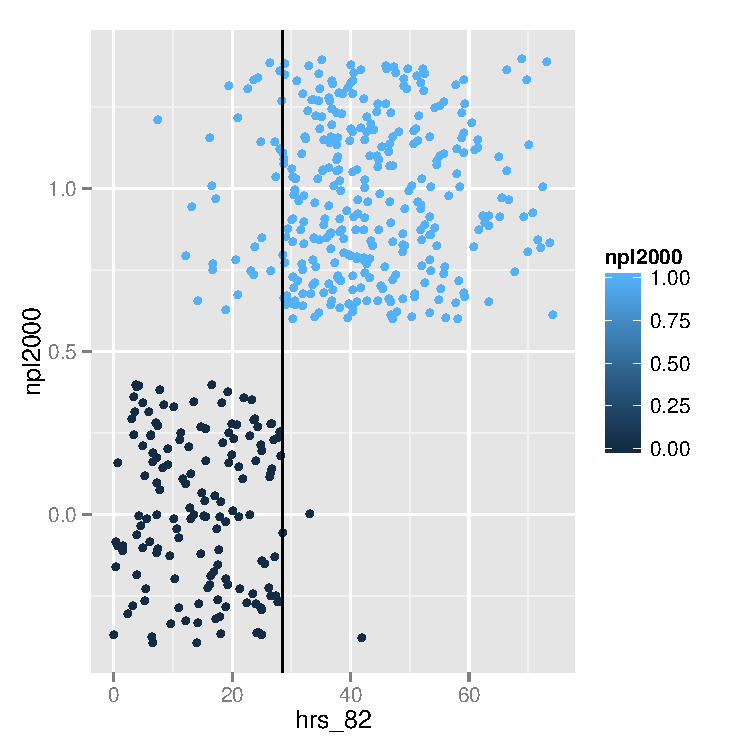
\includegraphics{fig-3b.pdf}
\caption{HRS score and status on NPL in 2000.  The points are jittered to indicate density; note that the actual values are either 1 or 0.}
\label{fig:3b}
\end{center}
\end{figure}

\subsection{Placebo Test}

Figure \ref{fig:3c} shows the influence of HRS on household values in 1980.  We would not expect any discontinuous jumps in this function because there was no cleanup initiated at that time.  This placebo test indicates there are not endogenous discontinuities in the value of households along the HRS scale.  

\begin{figure}[htbp!]
\begin{center}
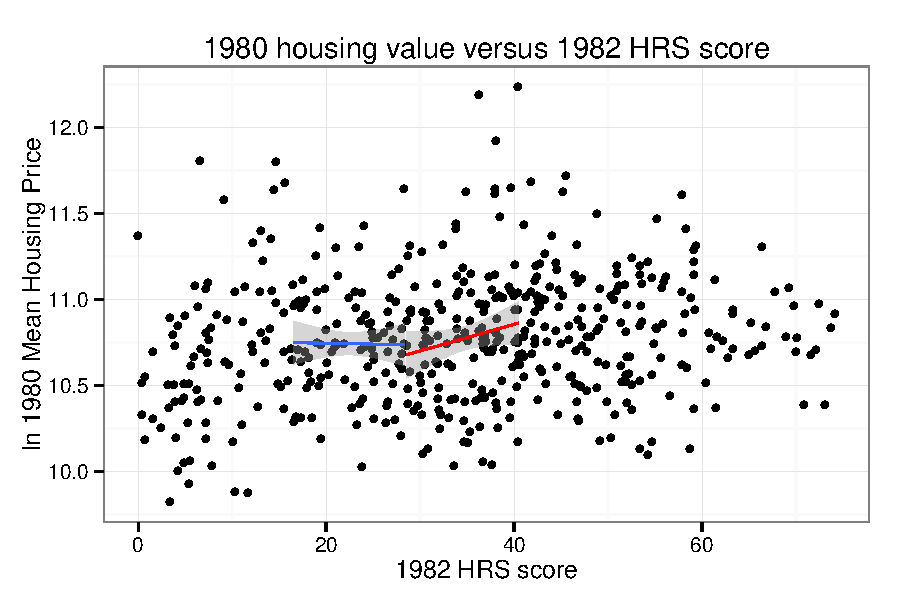
\includegraphics{fig-3c.pdf}
\caption{HRS score and 1980 mean property values.  There are local fit linear regressions on either side of the 28.5 cutoff in HRS.}
\label{fig:3c}
\end{center}
\end{figure}


\section{RDD Second Stage}

We use the reduced form for the second stage of IV estimation.  In this case, it is given by: 

$lnmdhsval0_{nbr}=\gamma_1\ind{HRS_{82} > 28.5} +\gamma_2(HRS_{82}-c) + \gamma_3(HRS_{82}-c)*\ind{HRS_{82} > 28.5}+x_i\gamma_4+u_i$.

For the IV to be valid there are two assumptions that need to be met: 1) the instrument needs to be correlated with treatment, which was shown to be true in the first stage equations above, and 2) the instrument should not be correlated with the error term, which is a reasonable assumption in this case based on the placebo test analysis above.  

While the first stage IV specification indicates a significant relationship between crossing the threshold and treatment status (both graphically and in the linear model formulation), the reduced form fails to show a relationship. We also used a plot more like the ones described in the notes (with local average values in evenly spaced bins and linear fits on either side of the threshold).  This is shown in figure \ref{fig:4b} below.  The result is the same as the plot with the full dataset, that there is not a discernible discontinuity in the data around the threshold.  The second stage fails to show any causal link between hazardous waste cleanup and housing values in the surrounding area, in spite of good specification of an instrument and a very strong first stage.  

\begin{figure}[htbp!]
\begin{center}
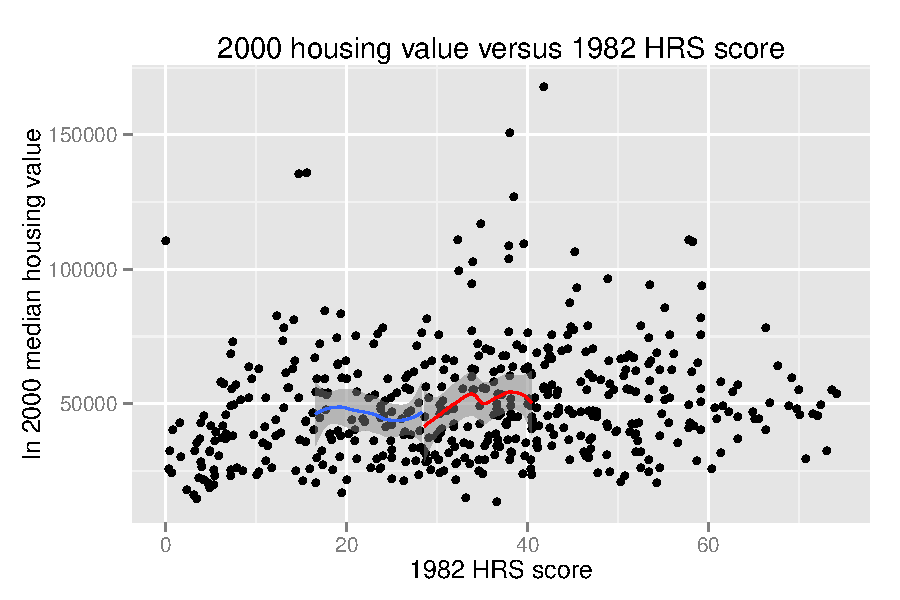
\includegraphics{fig-4.pdf}
\caption{HRS score and 2000 median property values.  There are local fit linear regressions on either side of the 28.5 cutoff in HRS.}
\label{fig:4}
\end{center}
\end{figure}

\begin{figure}[htbp!]
\begin{center}
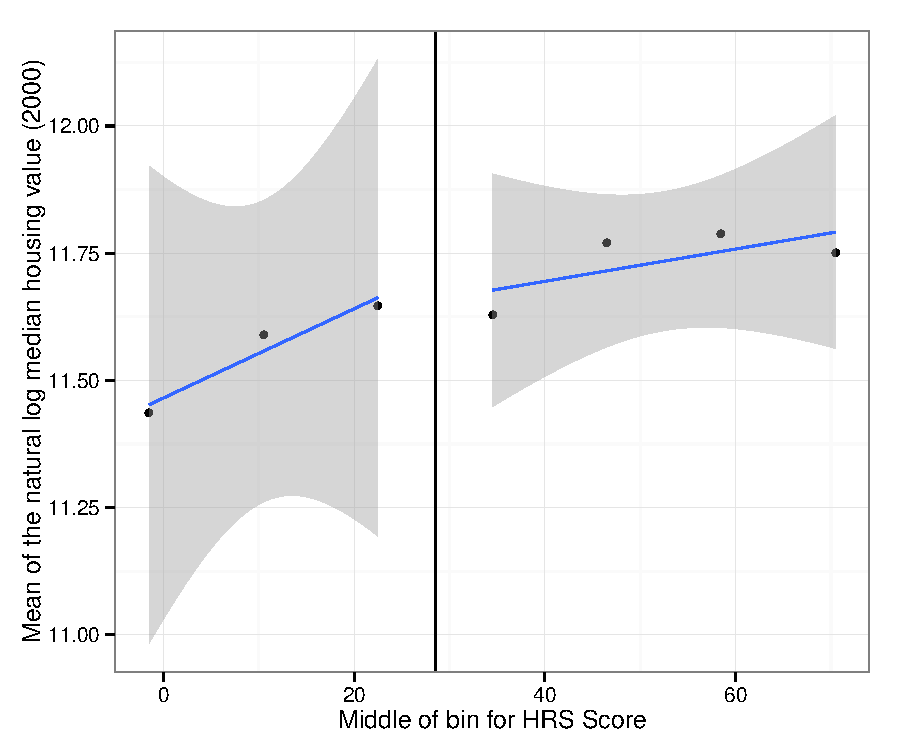
\includegraphics{fig-locavg-2000.pdf}
\caption{HRS score and 2000 median property values reported as the average in evenly spaced bins.  There are local fit linear regressions on either side of the 28.5 cutoff in HRS.}
\label{fig:4b}
\end{center}
\end{figure}

\subfile{tab3a.tex}

\section{Synthesis}

An ordinary least squares setup for estimating the effect of hazardous waste cleanup on housing prices indicates we should expect that sites with National Priorities List status result in higher home values than those not on the list---an increase in value from cleanup or the potential to have cleanup.  This approach is weak because it requires us to assume that we have a full set of observations for understanding the drivers of housing prices.  There also appear to be issues with overlap: there are significant differences between households in areas on NPL vs. those not on the list.  These differences seem to be less prominent as we narrow down on households close to the threshold for listing, motivating a regression discontinuity design.  By implementing a regression discontinuity design on the same data we can test whether this potential relationship holds up around the boundary of just-under or just-over the threshold for cleanup.    A well-structured RDD shows there is no relationship in the second stage despite a very strong first stage and no findings of manipulation.  In other words, the threshold for listing was as good as randomly assigned near the threshold, and does not have a noticeable effect on housing prices.  We trust the RDD more than OLS in this case because it is more robust in the face of error from unobserved housing characteristics and avoids overlap issues.  The findings from the OLS specification may be random error or some other unobserved characteristic manifesting as a higher value from NPL status.  Our overall finding is there is not apparent housing price benefit from NPL status.  

A potential confounding factor that is not addressed by either research design is the stigma that may be attached to ``superfund" sites.  By gaining NPL status, a site has access to cleanup money but also becomes known as a superfund site instead of just a ``normal" bazardous waste site.  For some people who may not trust the efficacy of cleanup efforts, they could exhibit a perverse aversion to superfund sites that are under cleanup to sites that just barely missed being labeled as superfund.

\section{Appendix: Code Listings}

\lstinputlisting{ps3.R}
\lstinputlisting{../util/are213-func.R}

\end{document}
